%Copyright 2019 Christopher M. Jermaine (cmj4@rice.edu) and Risa B. Myers (rbm2@rice.edu)
%
%Licensed under the Apache License, Version 2.0 (the "License");
%you may not use this file except in compliance with the License.
%You may obtain a copy of the License at
%
%    https://www.apache.org/licenses/LICENSE-2.0
%
%Unless required by applicable law or agreed to in writing, software
%distributed under the License is distributed on an "AS IS" BASIS,
%WITHOUT WARRANTIES OR CONDITIONS OF ANY KIND, either express or implied.
%See the License for the specific language governing permissions and
%limitations under the License.
\documentclass[aspectratio=169]{beamer}

%===============================================================%
\mode<presentation> 
{
\usetheme[noshadow, minimal,numbers,riceb,nonav]{Rice}
\usefonttheme[onlymath]{serif}
\setbeamercovered{transparent}
}
\useinnertheme{rectangles}

\usepackage[english]{babel}

\usepackage{mathptmx}
\usepackage{helvet}
\usepackage{courier}
\usepackage[T1]{fontenc}
\usepackage{trajan}

\setbeamerfont{block body}{size=\tiny}

%===============================================================%

\title[]
{Tools \& Models for Data Science}

\subtitle
{Course Overview}

\author[]{Risa Myers \& Chris Jermaine}
\institute
{
  Rice University
}

\date[]{}

\subject{Beamer}


\begin{document}

\begin{frame}
 \titlepage
\end{frame}

%***********************************************************

\begin{frame}{Welcome!}

\Large{Please fill out the questionnaire}
\vspace{1em}


\end{frame}
%***********************************************************

\begin{frame}{Welcome!}

\begin{itemize}
\item Introductions
\item Course overview
\item Syllabus / logistics
\item Tools
\end{itemize}
\end{frame}

%***********************************************************

\begin{frame}{Introductions!}

I am
\begin{itemize}
\item Risa Myers
\item Assistant Teaching Professor
\item rbm2@rice.edu
\item Duncan Hall  2062
\end{itemize}
\end{frame}

%***********************************************************

\begin{frame}{Who Are You?}

\Large{Trade questionnaires!}

\end{frame}

%***********************************************************

\begin{frame}{This Class is about \emph{Data Science}}

\begin{itemize}
\item What is THAT? 
\item Extraction of actionable knowledge from large volumes of data
	\begin{itemize}
	\item Encompasses methods from: 
		\begin{itemize}
		\item Computer science
		\item Statistics
		\item Optimization/Applied Math
		\end{itemize}
	\item Also includes
		\begin{itemize}
		\item Domain knowledge
		\item Communication skills
		\item Data management
		\end{itemize}

	\end{itemize}
    \end{itemize}
\end{frame}
%***********************************************************

\begin{frame}{Modern Data Scientists}

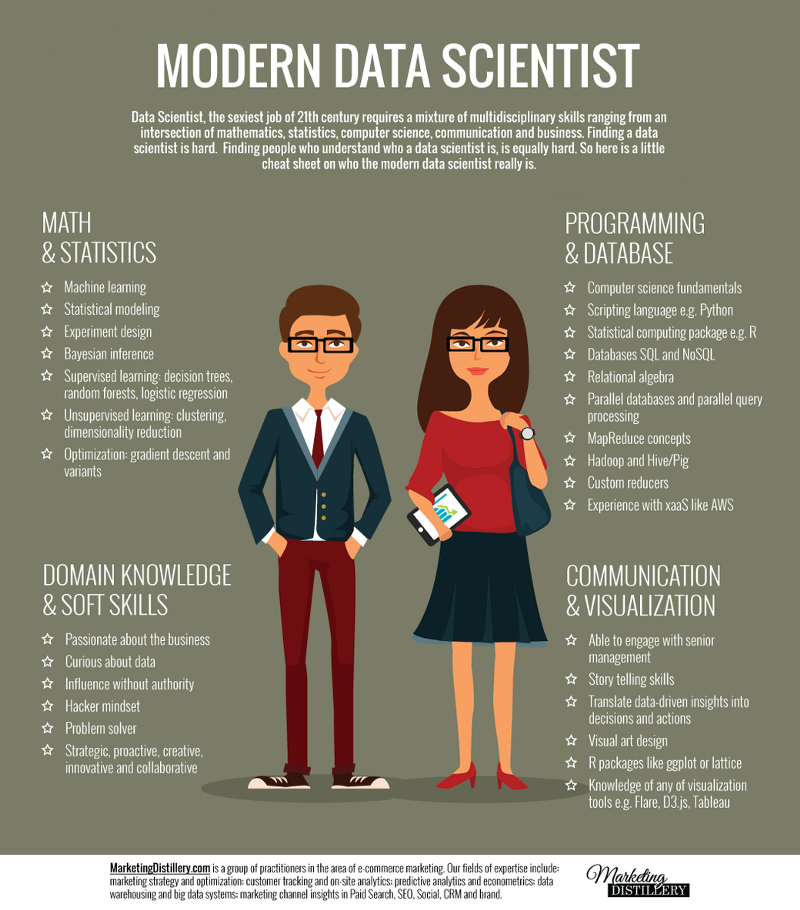
\includegraphics[width=.45\textwidth]{lectOverview/lookLike.png}

\end{frame}

%***********************************************************

\begin{frame}{Examples of Data Science Tasks}

\begin{itemize}
\item Given a huge set of per-customer sales data, build a model to predict customer ``churn''
\item Given a large graph of Medicare payout data, find suspicious (potentially fraudulent) referral patterns
\item Given a set of EMR data, find previously unknown side effects (ex: Vioxx and heart disease)
\item Given data from an online learning tool find markers that are an early sign of later academic achievement problems
\item Many, many more!
\end{itemize}
\end{frame}

%***********************************************************

\begin{frame}{Both Tools and Models are Important}
    \begin{itemize}
\item Back in the day...
	\begin{itemize}
	\item You had statisticians who dealt primarily with small data sets
	\item You had computer scientists who were interested in advanced modeling
	\end{itemize}
\item But in the ``Big Data'' era, the two can't live in isolation
	\begin{itemize}
	\item You need advanced models to solve challenging prediction/analysis tasks 
	\item You need computer systems that can scale those models to the largest data sets
	\item You need computer tools that make it easy to implement complicated models
	\end{itemize}
    \end{itemize}

\end{frame}
%***********************************************************

\begin{frame}{Important Disclaimer}
\begin{itemize}
\item Data Science Tools \& Models is fundamentally a computer science class!
\item This is not ``tools and models'' from a naive user's perspective
	\begin{itemize}
	\item No learning to be an end-user of classical analytics packages
	\item This is not a ``Get to know R'' class
	\item Nor is it a ``Get to know SAS'' class
	\item No plugging data into a standard software package and writing a report on the results
	\item A class covering such topics WOULD be useful
	\begin{itemize}
		\item But that's simply not this class
	\end{itemize}
	\end{itemize}
\item Lots of focus on algorithms and engineering

    \end{itemize}

\end{frame}

%***********************************************************

\begin{frame}{When We Say ``Models''} 
   \begin{itemize}
	\item Strong focus on the math foundations of data science
	\item Lots of optimization theory, probability, statistics
	\item Even some continuous mathematics
    \end{itemize}
\end{frame}
%***********************************************************


\begin{frame}{When We Say ``Tools''}
    \begin{itemize}
\item We mean tools for manipulating large data sets
\item Tools for scalable, distributed computation
\item Emphasis is on ``Big Data''!
\item Specifically, we'll learn about:
	\begin{itemize}
	\item SQL databases
	\item Python programming (NumPy, SciPy)
	\item Hadoop (MapReduce software, Big Data file system)
	\item Spark (distributed Big Data manipulation software)
	\end{itemize}
    \end{itemize}
\end{frame}
%***********************************************************

\begin{frame}{Example Use Case for Your  Data Science Tools \& Models Skill Set}
    \begin{itemize}
\item Imagine...
	\begin{itemize}
	\item You are working at a hospital
	\item You collect 5TB of patient monitoring data each day...
	\item And want a software to predict what will happen to a patient in the next hour
	\item Such a software does not exist...
	\item How to build it?
	\end{itemize}
\item Key questions to answer:
	\begin{itemize}
	\item How will you process the raw data?
	\item What model will you use to do prediction?
	\item How will you train the model?
	\item How will you scale to 5TB per day?
	\end{itemize}
\item After this class, you'll have the answers!    \end{itemize}
\end{frame}

%***********************************************************

\begin{frame}{As Such, this Class...}
    \begin{itemize}
\item Will give an introduction to modern data management software...
	\begin{itemize}
	\item First half of the class
	\item Relational database systems and SQL
	\item No-SQL systems such as Hadoop and Spark
	\end{itemize}
\item Will give an introduction to models for modern data analysis... 
	\begin{itemize}
	\item Second half of the class
	\item Supervised learning (linear models, support vector machines)
	\item Unsupervised learning (clustering, matrix factorization)
	\item Text mining
	\end{itemize}
\item Assignments will focus on implementing the models using the tools \& understanding methods for preparing data
    \end{itemize}

\end{frame}
%***********************************************************
\begin{frame}{Key Goals}

\begin{enumerate}
	\item Respect the data
\begin{itemize}
	\item Do good science
	\item Make repeatable processes
	\item Learn your data/domain
\end{itemize}
	\item Build your toolkit
	\item Know when to use the different tools \& models
	\item Learn to generalize
\begin{itemize}
	\item ``How can we use what we learned today?"
	\item ``What do we know now that we didn't know before?"
\end{itemize}
\end{enumerate}
\end{frame}


%***********************************************************

\begin{frame}{Skills You Need to Take this Class}
    \begin{itemize}
\item Should be a reasonable programmer
	\begin{itemize}
	\item Very comfortable with Python
	\item Two assignments use SQL (no knowledge assumed)
	\item Four assignments use Python
        \end{itemize}
    \end{itemize}
\end{frame}
%***********************************************************

\begin{frame}{More Skills You Need to Take this Class}

   \begin{itemize}
\item  Should not be afraid of a bit of math  
	\begin{itemize}
	\item Some background in probability/statistics
	\begin{itemize}
	\item Common distributions (e.g. Gaussian)
	\item Expected value
	\item Variance, covariance
	\item Norms (e.g. $L_1, L_2$)
	\end{itemize}
	\item Some calculus (partial derivatives \& the chain rule should not freak you out!)
	\item Linear algebra
	\begin{itemize}
	\item Vectors and scalars
	\item Matrix inversion
	\item Matrix transposition
	\item Dot products
	\end{itemize}
	\end{itemize}
    \end{itemize}
    

\end{frame}


%***********************************************************

\begin{frame}{Course Norms}
\begin{itemize}
\item If you don't understand something, say something... you're likely not the only one
\item No stupid questions
\item We may repeat lectures
\item We may adapt assignments
\item We may go over some basics that, depending on your background, might be review
\item If an assignment is taking too long, speak up! Get help! It may need to be changed
\end{itemize}
\end{frame}



%***********************************************************
\begin{frame}{What About Overlap with Other Classes?}

\begin{itemize}
\item COMP 330/543 and DSCI 302 -- biggest overlap
	\begin{itemize}
	\item Both may NOT be taken for credit
	\item COMP version is recommended for Computer Science majors
	\end{itemize}
\item COMP 430/533---significant overlap
\item COMP 440/502/540/602
	\begin{itemize}
	\item Many/all of the methods we'll cover will also be covered in those classes
	\end{itemize}
\end{itemize}
\end{frame}



%***********************************************************
\begin{frame}{Why take this class?}

\begin{itemize}
	\item To learn what Data Science is
	\item To develop familiarity and proficiency with common data science tools
\end{itemize}
\end{frame}

%***********************************************************
\begin{frame}{Class Syllabus}
\begin{itemize}
\item Communication...
\item Grading and Evaluation...
\item Exams...
\item Academic misconduct...
\item Assignments... 
\end{itemize}
\end{frame}
%***********************************************************
\begin{frame}{Logistics}
\begin{itemize}
\item Class
\begin{itemize}
\item MWF 9:00 - 9:50 PM
\item Location: TBD
\end{itemize}
\item Office Hours
\begin{itemize}
\item WF 10:00 - 11:00 AM
\item MWF 3:00 - 4:00 PM
\item Or by appointment
\item Duncan Hall 2062
\item TA Office Hours TBD
\item Watch Piazza for changes
\end{itemize}
\end{itemize}
\end{frame}

%***********************************************************
\begin{frame}{Communications}
\begin{itemize}
\item Canvas  \url{canvas.rice.edu}
\begin{itemize}
\item Assignments 
\item Grades
\item Lecture notes
\item Graded discussions
\end{itemize}
\item Piazza \url{tbd}
\begin{itemize}
\item Ungraded discussions
\end{itemize}
\item Email
\begin{itemize}
\item DSTM in subject line
\end{itemize}
\end{itemize}
\end{frame}
%***********************************************************
\begin{frame}{Assignments}

\begin{itemize}
\item Exercises
	\begin{itemize}
	\item 4 short programming or theory exercises designed to reinforce in-class concepts
	\end{itemize}
\item Labs
	\begin{itemize}
	\item 6 one-hour activities to get initial hands-on experience with a practical concept
	\end{itemize}
\item Programming Assignments
	\begin{itemize}
	\item 6 more in-depth programming assignments
	\end{itemize}
\end{itemize}
\end{frame}
%***********************************************************
\begin{frame}{Class Policies -- Due Dates}

\begin{itemize}
\item  \textbf{Assignment \& Exercise} Due Dates
\begin{itemize}
\item Typically due at 11:55 PM
\item Final assignment is due at the \textbf{end of the course final exam slot}
\item 1 second -- 24 hours late = 10\% penalty
\item 24 hours + 1 second -- 48 hours late = 20\% penalty
\item 48 hours + 1 second -- 72 hours late = 30\% penalty
\item > 72 hours late: NOT ACCEPTED
\item Last assignment may \textbf{NOT} be submitted late
\end{itemize}
\item Canvas is the time keeper -- if Canvas says it's late, it's late
\item Exceptions will only be made for EXTENDED Canvas outages
\item Submit early!
\end{itemize}
\end{frame}


%***********************************************************
\begin{frame}{Slip Days}

\begin{itemize}
\item 3 per person
\item Used in full day increments
\item Email me BEFORE the deadline
\item Once they are gone, they are gone
\item May NOT be used on final assignment
\end{itemize}
\end{frame}
%***********************************************************
\begin{frame}{Regrades}
\begin{itemize}
\item  Must be requested within 1 week of assignment/quiz  being returned
\item Intended for errors in grading or MINOR errors
\item Not a week-long extension to the assignment
\item Process
\begin{itemize}
\item Talk to Risa before class or during office hours
\item Write up request with complete details
\item Email to Risa with ``DSTM regrade''  subject
\end{itemize}
\end{itemize}
\end{frame}

%***********************************************************
\begin{frame}{Academic Misconduct}

\begin{columns}[t]
\begin{column}{0.5\textwidth}
\begin{itemize}
\item Rice Honor Code
\item On SOME assignments, you may share answers. Assume you may not. If it is permitted, it will be noted on the assignment.
\item No code sharing of ANY kind
\begin{itemize}
\item Email
\item Whiteboard
\item Sharing / showing your screen
\item Piazza posts
\item Verbally
\end{itemize}
\end{itemize}
\end{column}
\begin{column}{0.5\textwidth} 
\begin{itemize}
\item No outside help
\begin{itemize}
\item No StackOverflow posting
\item No Googling solutions
\item No asking someone who took the class last year/semester
\end{itemize}
\item ``2 line rule''
\item  OK (encouraged) to look up syntax
\end{itemize}
\end{column}
\end{columns}
\end{frame}


%***********************************************************

\begin{frame}{Questions?}

\begin{itemize}
\item If there's time: on to data
\end{itemize}

\end{frame}

\end{document}
